\documentclass[11pt]{article}
\usepackage{geometry,marginnote} % Pour passer au format A4
\geometry{hmargin=1cm, vmargin=1cm} % 

% Page et encodage
\usepackage[T1]{fontenc} % Use 8-bit encoding that has 256 glyphs
\usepackage[english,french]{babel} % Français et anglais
\usepackage[utf8]{inputenc} 

\usepackage{lmodern,numprint}
\setlength\parindent{0pt}

% Graphiques
\usepackage{graphicx,float,grffile}
\usepackage{pst-eucl, pst-plot,units} 

% Maths et divers
\usepackage{amsmath,amsfonts,amssymb,amsthm,verbatim}
\usepackage{multicol,enumitem,url,eurosym,gensymb}
\DeclareUnicodeCharacter{20AC}{\euro}

% Sections
\usepackage{sectsty} % Allows customizing section commands
\allsectionsfont{\centering \normalfont\scshape}

% Tête et pied de page
\usepackage{fancyhdr} \pagestyle{fancyplain} \fancyhead{} \fancyfoot{}

\renewcommand{\headrulewidth}{0pt} % Remove header underlines
\renewcommand{\footrulewidth}{0pt} % Remove footer underlines

\newcommand{\horrule}[1]{\rule{\linewidth}{#1}} % Create horizontal rule command with 1 argument of height

\newcommand{\Pointilles}[1][3]{%
  \multido{}{#1}{\makebox[\linewidth]{\dotfill}\\[\parskip]
}}

\newtheorem{Definition}{Définition}

\usepackage{siunitx}
\sisetup{
    detect-all,
    output-decimal-marker={,},
    group-minimum-digits = 3,
    group-separator={~},
    number-unit-separator={~},
    inter-unit-product={~}
}

\setlength{\columnseprule}{1pt}

\begin{document}


\section*{Semaine 4 - The insides of giant planets (week 1)}


\begin{itemize}[label={$\bullet$}]
    \item Vidéo : 2.01: Introduction to Jupiter
    \item Vidéo : 2.02: Measuring density
    \item Demande de discussion : Transit of Venus!
    \item Vidéo : 2.03: Using density
    \item Vidéo : 2.04: Hydrostatic equilibrium
    \item Vidéo : 2.05: Hydrogen equation of state
    \item Vidéo : 2.06: Heat transport
    \item Vidéo : 2.07: Theoretical internal structure
    \item Vidéo : 2.08: A core from gravity ?
    \item Vidéo : 2.09: Magnetic fields
    \item Vidéo : 2.10: The upper atmosphere and the Galileo probe
    \item Vidéo :2.11: Picture models
\end{itemize}

\subsection*{Quiz 4}

\begin{enumerate}
    \item[1.] Kepler's planetary laws, coupled with Newton's equation of 
    gravitation, lets us determine the mass of a planet by measuring the 
    orbital semimajor axis and orbital period. 
    
    Which one of the 
    following moons will have almost exactly the same period as a moon with the mass of Europa $1 M_e$ with a semimajor axis of 1 million km  $10^6 km$ around a planet with the mass of Jupiter $1 M_J$
    
    A moon with a mass of $(in M_e)$, a semimajor axis of (in km), and orbital a planet with the mass of in $(M_J)$:
    \begin{itemize}[label={$\bullet$}]
        \item moon mass = $2 M_e$ ; semi axis = $2 \times 10^6 km$ ; planet mass = $8 M_j$
        \item moon mass = $1/2 M_e$ ; semi axis = $1/2 \times 10^6 km$ ; planet mass = $8 M_j$
        \item moon mass = $1/2 M_e$ ; semi axis = $2 \times 10^6 km$ ; planet mass = $2 M_j$
        \item moon mass = $1 M_e$ ; semi axis = $1/2 \times 10^6 km$ ; planet mass = $2 M_j$
        \item moon mass = $1/2 M_e$ ; semi axis = $8 \times 10^6 km$ ; planet mass = $2 M_j$
        \item moon mass = $1 M_e$ ; semi axis = $1/8 \times 10^6 km$ ; planet mass = $1/2 M_j$
    \end{itemize}

    \item[2.] Of the planets in the solar system Earth is the most dense and Saturn is the least dense, but the densities of the planets are greatly affected  by compression. Planetary scientist often talk of "uncompressed densities" meaning the density that the planet would have if all of its materials were at 1 bar of pressure. Using what you know of the densities of materials and the compositions of the planets, which planet has the highest uncompressed density?
    \begin{multicols}{4}
    \begin{itemize}[label={$\bullet$}]
       \item Mercury
       \item Venus
       \item Earth
       \item Mars
       \item Jupiter
       \item Saturn
       \item Uranus
       \item Neptune
    \end{itemize}
\end{multicols}
    \item[3.]     The equation of hydrostatic equilibrium allows you to determine the pressure inside of a planet as a function of depth. 
    What piece of information is required in all cases to use the equation of hydrostatic equilibrium?
    
    \begin{itemize}[label={$\bullet$}]
        \item A knowledge of whether or not there is a core inside of the planet.
        \item An equation of state telling you the density of the material as a function of pressure.
        \item The temperature profile inside of the planet.
        \item A phase diagram of the substance at the temperatures and pressures of the interior.
        \item The mean molecular mass of the substance
        \item An understanding of the interior heat flow.
    \end{itemize}
    

    \item[4.] In a Fermi gas -- which is not a bad approximation to the equation of state in the center of Jupiter -- what is the main reason for the resistance of the gas to compression?
    \begin{multicols}{4}
    \begin{itemize}[label={$\bullet$}]
        \item Electrons which are unable to occupy the same quantum state.
        \item Electrostatic repulsion
        \item High temperatures
        \item A high effective mean molecular mass
        \item A phase transition to a solid
        \item Convective instability
    \end{itemize}
\end{multicols}

    \item[5.] Which of the following is the farthest from being in hydrostatic equilibrium? (notice that I say farthest here, because new things are perfectly in hydrostatic equilibrium, but many things are pretty close).
    
    \begin{itemize}[label={$\bullet$}]
        \item The water inside of a glass
        \item The interior of the Earth
        \item The interior of Jupiter
        \item The Earth's atmosphere
        \item A rock
    \end{itemize}

    \item[6.] Which of the following is NOT true about the process of convection?
    \begin{itemize}[label={$\bullet$}]
        \item Convection can occur due to cooling at the top as well as heating at the bottom.
        \item Convection of a conducting medium is required for the generation of a magnetic field inside of a planet      
        \item Convection is the fastest way for a planet to remove heat from its interior
        \item Convection can only be sustained if energy is both input at the bottom and removed at the top.
        \item These are all true
        \item Any time warm air is below cooler air, convection will occur
    \end{itemize}
    \item[7.] We think Jupiter most likely has a core, though it is one of the major goals of the Juno spacecraft to find out for sure. Which of the following is NOT a reason that we think Jupiter most likely has a core?

    \begin{itemize}[label={$\bullet$}]
        \item To fit the density of Jupiter you need to add a significant amount of extra heavier material compared to the atmosphere.
        \item Saturn clearly has a core and  it would seem odd to have two planets right next to each other and that look so similar to actually be so different on the inside.
        \item The best fit interior models, though still uncertain, work better with a core than without.
        \item The presence of a magnetic field strong suggests the presence of a core
        \item All of these are reasons to think that Jupiter has a core
    \end{itemize}
    

    \item[8.] Which of the following is a TRUE statement about what was found by sending the Galileo probe into Jupiter?

\end{enumerate}
\begin{multicols}{2}
\begin{itemize}[label={$\bullet$}]
    \item None of these is true
    \item The chemicals in the atmosphere of Jupiter are spatially homogeneous 
    \item The upper atmosphere has elevated abundances of many elements
    \item The abundances of helium and neon are elevated because they are retained in clouds in the upper atmosphere 
    \item Water vapor is abundant just below the cloud tops
\end{itemize}
\end{multicols}

\newpage 

\section*{Semaine 5 - The insides of giant planets (week 2)}


\begin{itemize}[label={$\bullet$}]
    \item Vidéo : 2.12: Planetesimal formation
    \item Vidéo : 2.13: Core formation
    \item Vidéo : 2.14: Core-collapse vs. Disk instability
    \item Demande de discussion : Core collapse vs. disk instability?
    \item Vidéo : 2.15: Saturn and the ice giants
    \item Vidéo : 2.16: Discovering hot Jupiters
    \item Vidéo : 2.17: Densities of hot Jupiters
    \item Vidéo : 2.18: Inflating hot Jupiters
    \item Vidéo : 2.19: Kepler and the sub-Neptunes
    \item Vidéo : 2.20: Exoplanet spectroscopy
    \item Vidéo : 2.21: Juno and future exploration
    \item Demande de discussion : Juno results?
\end{itemize}

\newpage 

\subsection*{Quiz 5}

\begin{enumerate}
\item[1.] Which planet would have the lowest uncompressed density?
    \begin{multicols}{4}
    \begin{itemize}[label={$\bullet$}]
        \item Mercury
        \item Venus
        \item Earth
        \item Mars
        \item Jupiter
        \item Saturn
        \item  Uranus
        \item  Neptune
    \end{itemize}
    \end{multicols}

\item[2.] Which of the following is  not  a reason that we expect metallic hydrogen inside of Jupiter?
    \begin{multicols}{2}   
    \begin{itemize}[label={$\bullet$}]
        \item The phase diagram predicts metallic hydrogen.
        \item All of these statements are true.
        \item Helium rains out of the upper layers into the lower layers.
        \item The presence of a strong magnetic field suggests a conductive interior.
        \item The dipole nature of the magnetic field suggests a deep conductive layer
        \item The interior pressures are higher than the gas-to-metal transition.
    \end{itemize}
    \end{multicols}

\begin{multicols}{2}  
\item[3.] Which of the following orbits (some of which would require extra propulsion to follow) would be best for using gravitational measurements to determine the interior structure of a planet? (the inner and outer dashed lines are circles of 10 planet radius and 100 planet radius, for consistent scale)
    \begin{figure}[H]
        \centering
        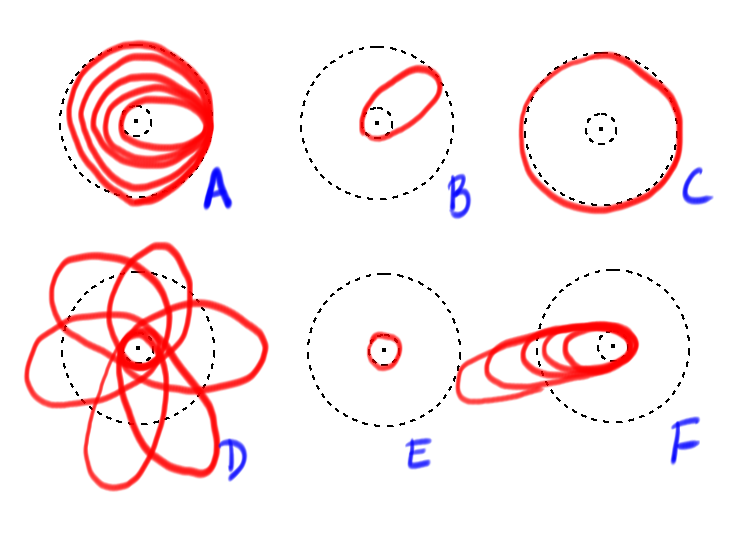
\includegraphics[width=0.8\linewidth]{orbits.png}
    \end{figure}
\end{multicols}

\item[4.] Which of the following is not required for the creation of a dynamo-driven magnetic field?
    \begin{multicols}{2}
    \begin{itemize}[label={$\bullet$}]
        \item Interior motions deflected by the Coriolis effect
        \item A core of ice and/or rock
        \item A rotating planet
        \item All of these are required
        \item A conducting liquid in the interior
        \item An interior which gets hotter with depth
        \item Convection in the interior
    \end{itemize}
\end{multicols}

\item[5.] Which of the following is the best description of the formation of a giant planet with a massive core? (at least as described in the lectures!)
    
    \begin{itemize}[label={$\bullet$}]
        \item In a massive disk the force of gravity in a patch of the disk overcomes the pressure and rotational forces and the patch quickly collapses into a giant planet. The heavy materials sink to the bottom and form the core.
        \item Planetesimals grow through gravitational focusing. Dynamical friction slows the motions of the largest objects leading to runaway growth of oligarchs, which are isolated from other nearby oligarchs. The gravitational pull of the oligarch quickly overcomes the rotational and pressure forces from the disk, causing rapid growth of the gaseous atmosphere.
        \item Planetesimals grow through gravitational focusing. Dynamical friction slows the motions of the largest objects leading to runaway growth of oligarchs, which are isolated from other nearby oligarchs. Gas slowly accretes onto the oligarch through an envelope until the pressures are too high to support the envelope and massive amounts of gas collapse making the gas giant.
        \item Planetesimals grow through gravitational focusing. Dynamical friction speeds the motions of the largest objects leading to more frequent collisions and runaway growth of oligarchs, which are isolated from other nearby oligarchs. Gas slowly accretes onto the oligarch through an envelope until the pressures are too high to support the envelope and massive amounts of gas collapse making the gas giant.
        \item Planetesimals grow through gravitational focusing. Dynamical friction slows the motions of the largest objects leading to runaway growth of oligarchs, which are isolated from other nearby oligarchs. Large numbers of oligarchs merge over hundreds of millions of years, leading to a giant core.Gas slowly accretes onto the oligarch through an envelope until the pressures are too high to support the envelope and massive amounts of gas collapse making the gas giant.
    \end{itemize}

\item[6.] Based on our current understanding of the results from the Kepler mission, what is the most common type of planet with orbital periods less than 90 days?
    \begin{multicols}{3}
    \begin{itemize}[label={$\bullet$}]
        \item Planets with masses between that of the Earth and Neptune
        \item Hot Jupiters
        \item Water worlds
        \item Super earths with solid surfaces
        \item Planets less massive than the Earth
        \item Sub-Neptunes with ice/rock cores and gas envelopes
    \end{itemize}
\end{multicols}

\item[7.] The processes of gravitational focusing and dynamical friction are critical to our understanding of how planetesimals form. Which of the following is NOT true about gravitational focusing and dynamical friction?

    \begin{itemize}[label={$\bullet$}]
        \item As dynamical friction slows down large bodies with respect to each other, gravitational focusing increases dramatically
        \item  Dynamical friction makes small bodies go fast and large bodies go slow
        \item Dynamical friction works most efficiently when all of the bodies are approximately the same size
        \item All of these statements are true
        \item Gravitational focusing gets much stronger for bodies that are nearly motionless with respect to each other
        \item Gravitational focusing gets stronger for larger bodies
    \end{itemize}
    

\item[8.] Isolation mass is another key concept in understanding the formation of planetesimals and eventually planets. We sometimes use the term "oligarch" to describe a body which has become isolated. Which of the following statements about isolation mass is false?
    \begin{multicols}{2}
    \begin{itemize}[label={$\bullet$}]
        \item Oligarchs are space further and further apart further out in the dis
        \item Isolation masses are much higher outside of the ice line
        \item Dynamical friction causes the oligarchs to slow each other down
        \item When an object reaches isolation mass it stops growing rapidly by gravitational focusing  
        \item Oligarchs get more massive futher out in the disk
        \item All of these statements are true
    \end{itemize}
    \end{multicols}

\item[9.] While we think that our planets formed through the process of core collapse, planets around other stars might or might not have formed from the process of disk instability. Which of the following would make disk instability MORE LIKELY to have occurred around a star?
    \begin{multicols}{3}
    \begin{itemize}[label={$\bullet$}]
        \item A hotter  disk of material
        \item A more massive disk
        \item A more massive star
        \item A larger fraction of solid material in the disk
        \item A previously formed planet
        \item None of these would make disk instability more likely
    \end{itemize}
    \end{multicols}

\item[10.] Uranus and Neptune are very different from Jupiter and Saturn. Which of the following is NOT true of the differences between these sets of planets?
    \begin{multicols}{2}
    \begin{itemize}[label={$\bullet$}]
        \item Uranus and Neptune are more dense than Jupiter and Saturn, even though Jupiter and Saturn are much more compressed.
        \item While Jupiter and Saturn have mostly regular magnetic fields, the complex non-dipolar magnetic fields of Uranus and Neptune suggest that the magnetic field is generating closer to the top of the atmosphere on these planets.
        \item Uranus and Neptune have only a fraction of the mass of Jupiter or Saturn
        \item All of these statements are true
        \item Neither Uranus nor Neptune is massive to have metallic hydrogen on the inside
    \end{itemize}
    \end{multicols}                    
\end{enumerate}



\newpage 

\section*{Semaine 6 - Big questions from small bodies}


\begin{itemize}[label={$\bullet$}]
    \item 3.01: Introduction to the small bodies of the solar system
    \item 3.02: The formation of small bodies
    \item 3.03: The formation of terrestrial planets
    \item 3.04: The surface density of the solar system
    \item 3.05: An ode to comets
    \item 3.06:The composition of comets
    \item 3.07: Where do comets come from?
    \item 3.08: The formation of the Oort cloud
    \item 3.09: Meteorites and the beginning of the solar system
    \item 3.10 Types of meteorites: Chondrites
    \item 3.11: Types of meteorites: Achondrites
    \item 3.12: Asteroids and meteorite delivery
\end{itemize}

\newpage 

\subsection*{Quiz 6}

\begin{enumerate}
    \item[1.] Which of the following is the best explanation of why we have small bodies in the solar system?
    \begin{multicols}{2} \begin{itemize}[label={$\bullet$}]
        \item The oligarchs that formed in the region of the terrestrial planets and the asteroid belt slowly merged over ~100 Myr and the oligarchs at the outer range of this region were excited by Jupiter enough to cause impacts to shatter the objects. A similar process took place in the Kuiper belt.
        \item Planetesimal formation in the region of the asteroid and Kuiper belts was delayed until after the gas in the nebular disk had dissipated, preventing these objects from acquiring gassy envelopes.
        \item Insufficient mass existed in the region of the asteroid belt and Kuiper belt to allow full sized planets to form.
        \item Nearby planets caused excitation of the orbits of planets in the region of the asteroid belt and Kuiper belt and these planets collided and their fragments are now the small bodies.
        \item Nearby planets caused the orbits of forming planetesimals to acquire high velocities and eccentricities, preventing run away growth and leading to shattering impacts.
    \end{itemize}\end{multicols}       

    \item[2.] Which of the following statements about comets is NOT true?
    \begin{multicols}{2} \begin{itemize}[label={$\bullet$}]
        \item Water is the most abundant ice on comets and the most abundant gas in the coma of a comet
        \item All of these statements about comets are true      
        \item Much of the light we see in the coma of a comet is sunlight reflected off of an extended dust coma lifted off the surface
        \item Comets typically become bright at distances of about 3 AU from the sun where water ice begins to sublime
        \item Comets have slight deviations in their orbits when they get close to the sun due to the jetting effect of evaporation
        \item The ices present in comets show that these bodies were formed in the regions beyond Jupiter
    \end{itemize}\end{multicols}      
    \item[3.] Which of the following is NOT required for the formation of a large nearly isotropic Oort cloud full of many small bodies, assuming the scenario that we discussed is the dominant mechanism? 
    \begin{multicols}{2} \begin{itemize}[label={$\bullet$}]
        \item A planet like Jupiter which is massive enough to scatter bodies out of the solar system
        \item Passing stars which perturb the orbits of low perihelion, high semimajor axis objects      
        \item A smaller planet like Neptune to scatter icy bodies inward so they can be ejected by a more massive planet like Jupiter
        \item A population of small bodies which is close enough to a planet to get scattered outward
        \item Multiple stellar encounters to randomize the cometary orbits into an isotropic cloud
        \item All of these are required
    \end{itemize}\end{multicols}   
    \item[4.] The terrestrial planets appear to have taken much longer to finally assemble than the gas giants did. Which of the following statements about these timescale is NOT true?
    \begin{multicols}{2} \begin{itemize}[label={$\bullet$}]
        \item We can learn about the timescale of terrestrial planet differentiation by looking at isotopic ratios of hafnium and tungsten.
        \item Mars differentiated quickly, so tungsten-182, the radioactive decay product of hafnium, is abundant in Martian meteorites.       
        \item One reason that the gas giant formation timescale is thought to be so fast is that we do not observe stars to have gas around them after they are ~3 Myr old
        \item Growth of the terrestrial planets was slowed by the rapid growth of the gas giants, which caused oligarchs to have have velocities and break apart.
        \item All of these statements are true
        \item Oligarchs form very quickly through runaway growth but because they are gravitationally isolated it takes a long time for them to assemble into larger bodies.
    \end{itemize}\end{multicols}   
    \item[5.] The "minimum mass solar nebula" shows how much initial mass was needed in the disk around the sun to form the planets that we know of today. Which statement about the minimum mass solar nebula below is FALSE?
    \begin{multicols}{2} \begin{itemize}[label={$\bullet$}]
        \item WAll of these are true
        \item The minimum mass solar nebula approximately accounts for all of the hydrogen and helium that were present in the initial disk but which were not incorporated into the terrestrial planets.      
        \item Mars appears to have less mass than would be predicted by a smooth minimum mass solar nebula 
        \item The initial distribution of mass in the solar system could have been very different from that reconstructed in the "minimum mass solar nebula"
        \item The disk of material around the sun could have had more material than the minimum mass solar nebula
    \end{itemize}\end{multicols}   
    \item[6.] Which of the following is NOT part of the explanation for why we continue to have near earth asteroids hit the earth even though the dynamical lifetime of a typical NEA is very short compared to the age of the solar system? (by dynamical lifetime we mean the time before it is likely to hit a planet or get ejected from the solar system) 
    \begin{multicols}{2} \begin{itemize}[label={$\bullet$}]
        \item The existence of families of asteroids formed by asteroid impact and shattering
        \item The high current eccentricities and inclinations of asteroids population leading to shattering impacts       
        \item All of these are true
        \item The Yarkovsky effect
        \item Heating of small asteroids on one side coupled with rotation causing orbital drift
        \item Our improved technology which allows us to find ever-smaller near earth asteroids
        \item Resonances with Jupiter and Saturn in the asteroid belt leading to removal of objects in the asteroid belt
    \end{itemize}\end{multicols}   
    \item[7.]Lead-lead dating is a great way to figure out the age of something that is close to the age of the solar system. It based on the radioactive decay of uranium.Uranium-238 decays (with intermediate steps) to lead-206 with a half life of 4.5 billion years. Uranium-235 decays to lead-207 with a half life of 0.7 billion years.
    \begin{multicols}{2} \begin{itemize}[label={$\bullet$}]
        \item A higher ratio of lead-204 to lead-206 implies a younger rock
        \item Measuring the abundance of uranium-235 shows you how many half-lives have passed since the formation of the rock
        \item The technique requires finding parts of the meteorite with different abundances of lead and trying to determine how much extra lead exists because of uranium decay
        \item Objects which are younger will have more lead-207 than objects which are older.
    \end{itemize}\end{multicols}   
    \item[8.] We find chondrules in meteorites that fall from the sky, but we have never found them on the Earth, the Moon, or Mars. Why not?
    \begin{multicols}{2} \begin{itemize}[label={$\bullet$}]
        \item They are in the interior of the Earth where we cannot reach.
        \item None of these is correct
        \item Meteorites probably formed from different materials than the planets
        \item They most likely form as the meteorite is falling through the atmosphere
        \item Materials inside large bodies like the Earth, Moon, and Mar undergo so much transformation due to heat and pressure that their original structure is not preserved.
    \end{itemize}\end{multicols}   
    \item[9.]  Pallasites are not only once of the most beautiful types of meteorites that you can find, they are also one of the most special. Many things must happen before a pallasite can form and be delivered to your hand. Which of the following is NOT one of them?
    \begin{multicols}{2} \begin{itemize}[label={$\bullet$}]
        \item Someone has to find the pallasite on the Earth (and, eventually, it gets handed to you)
        \item A body must form which is large enough to retain enough heat to differentiate
        \item Pieces of a shattered body must hit a resonance which puts them onto an Earth crossing orbit
        \item All of these must happen
        \item A differentiated body must have an impact which shatters it into pieces
        \item A piece of the core-mantle boundary from a shattered mini-planet must land on the Earth
    \end{itemize}\end{multicols}   
\end{enumerate}

\newpage 

\section*{Semaine 7 - Big questions from small bodies}


\begin{itemize}[label={$\bullet$}]
    \item 3.13: Asteroid compositions
    \item 3.14: Pictures of asteroids
    \item 3.15: Asteroid hazards
    \item 3.16: The Kuiper belt
    \item 3.17: Properties of dwarf planets
    \item 3.18: Dynamical instabilities
    \item 3.  : Lucy!
    \item 3.19: The Grand Tack
    \item 3.20: Planet Nine
    \item 3.21:  A trip to the Subaru telescope
\end{itemize}

\newpage 

\begin{enumerate}
    \item[1.] Put the following in order from earliest to latest. In doing so, assume that the Nice model occurred as described and that the Grand Tack model also occurred as described.
    \begin{multicols}{2} \begin{itemize}[label={$\bullet$}]
        \item The formation of Jupiter 
        \item The inward migration of Jupiter due to gas forces 
        \item The instability "explosion" which scattered small bodies throughout the solar system
        \item The inward migration of Saturn due to gas forces 
        \item The formation of the Earth
        \item The outward migration of Jupiter due to gas forces 
        Be very careful typing in your answer! If you think the order is 1,2,3,4,5,6 please type, exactly "123456" with no spaces, no commas, and no quotation marks.
    \end{itemize}\end{multicols}   
    \item[2.] What problem does the Grand Tack model of the early solar system evolution attempt to explain?
    \begin{multicols}{2} \begin{itemize}[label={$\bullet$}]
        \item The continued delivery of near earth asteroids into the inner solar system.
        \item The early inward migration of Jupiter and Saturn
        \item The mixing of the asteroid belt
        \item The timing of the Late Heavy Bombardment
        \item The apparently low mass of Mars
        \item The number of terrestrial planets
    \end{itemize}\end{multicols}
    \item[3.] For lead-lead dating, we measure the ratio of 207Pb to 206Pb and the ratio of 204Pb to 206Pb in a series of different regions of a meteorite. We then construct a plot of all of our measurements which looks something like this. The individual measurements are the points labeled things like "L1" and "W8"; a line is drawn through the points. The line is defined by a slope and the location where it hits the y-axis (the "intercept"), which is about 0.62 in this case. If we made similar plots for each of a series of calcium aluminum inclusions (CAIs) and a collection of chondrites, what are we most likely to find?
    \begin{multicols}{2} \begin{itemize}[label={$\bullet$}]
        \item The slopes measured for the CAIs would all be nearly identical, while the slopes measured for the chondrites would range from that of the CAIs to larger (steeper) values
        \item The slope of each measured line would be nearly identical. The intercepts for the CAIs would all be equal, and the intercepts for the chondrites would range from that of the CAI to larger values.
        \item The slopes measured for the CAIs would all be nearly identical, while the slopes measured for the chondrites would all be smaller (shallower)
        \item The slopes measured for the CAIs would all be nearly identical, while the slopes measured for the chondrites would range from that of the CAIs to smaller (shallower) values
        \item The slopes measured for the CAIs would all be nearly identical, while the slopes measured for the chondrites would all be larger (steeper).
        \item The slope of each measured line would be nearly identical, but the intercepts for the CAIs would all be smaller than the intercepts for the chondrites.
        \item The slope of each measured line would be nearly identical. The intercepts for the CAIs would all be equal, and the intercepts for the chondrites would range from that of the CAI to smaller values. 
    \end{itemize}\end{multicols}
    \item[4.] What can not we infer from this plot of the eccentricity vs. semimajor axis of known Kuiper belt objects?
    \begin{multicols}{2} \begin{itemize}[label={$\bullet$}]
        \item Neptune may have migrated outward, pushing parts of the Kuiper belt outward
        \item No objects with circular orbits are known beyond the 2:1 resonance with Neptune
        \item Many Kuiper belt objects share identical orbital periods as Pluto
        \item Kuiper belt objects have had giant impacts which have made families
        \item Kuiper belt objects exist out to at least ~180 AU
        \item Neptune is currently scattering Kuiper belt objects
    \end{itemize}\end{multicols}
    \item[5.] What is the explanation for the apparent lack of abundant solid nitrogen on the surface of Makemake even though it dominates the surface of Pluto and is inferred to be present on Eris?
    \begin{multicols}{2} \begin{itemize}[label={$\bullet$}]
        \item MThe saturated spectrum of the slabs of methane make nitrogen too difficult to detect.
        \item MMakemake is warmer than Eris but colder than Pluto, allowing methane to be stable but not nitrogen
        \item MMakemake is colder than Pluto, so nitrogen is frozen on the surface and not detected in the atmosphere
        \item MMakemake is smaller than Pluto and Eris, so nitrogen escapes while the less volatile methane remains behind.
        \item MMethane is so abundant on Makemake that chemical reactions between methane and nitrogen make ammonia
        \item MMakemake is smaller than Pluto and Eris, so molecular nitrogen undergoes hydrodynamic escape while leaving the lighter methane molecule behind
    \end{itemize}\end{multicols}
    \item[6.] Is Pluto a planet?
    \begin{multicols}{2} \begin{itemize}[label={$\bullet$}]
       \item yes
       \item no
    \end{itemize}\end{multicols}
    \item[7.] Which of the following is not a possible consequence of the Nice model for the dynamical instability of the early solar system? 
    \begin{multicols}{2} \begin{itemize}[label={$\bullet$}]
       \item The small mass of the Kuiper belt
       \item The presence of icy bodies among the Jupiter trojan
       \item The abundance of Kuiper belt objects in resonaces
       \item The low mass of Mars
       \item The higher than expected eccentricities of the giant planets
       \item The lateness of the Late Heavy Bomdardment
    \end{itemize}\end{multicols}
    \item[8.] Is it possible that a civilization destroying asteroid is going to hit us within the next century?
    \begin{multicols}{2} \begin{itemize}[label={$\bullet$}]
        \item yes
        \item no
     \end{itemize}\end{multicols}
    \item[9.] Which of the following statements about the hypothetical Planet Nine is NOT true?
    \begin{multicols}{2} \begin{itemize}[label={$\bullet$}]
        \item In the Planet Nine model, Planet Nine clears out the majority of the high eccentricity high semimajor axis objects in the outer solar system
        \item All of these are true
        \item Planet Nine can raise the perihelion of objects like Sedna and 2012 VP113
        \item Planet Nine finally explains the discrepancies in the orbital position of Neptune
        \item Pluto was originally though to be possibly as large as Jupiter
        \item In the Planet Nine model, Planet Nine tilts the orbits of distant eccentric Kuiper belt objects into a plane different from the plane of the planets.
    \end{itemize}\end{multicols}
    \item[10.] NASA is planning to send the Lucy spacecraft to study Trojan asteroids in the next decade. What of the following statements about Trojan asteroids is TRUE? Check all that apply. 
    \begin{multicols}{2} \begin{itemize}[label={$\bullet$}]
        \item In the Nice dynamical instability model, Trojan asteroids and Kuiper belt objects come from the same source
        \item It is possible that Trojan asteroids formed in the asteroid belt
        \item Trojan asteroids are dynamically unstable on ~1 million year lifetimes so must be replenished by asteroid collisions.
        \item Trojan asteroids look different spectroscopically from the majority of the asteroids in the main asteroid belt
    \end{itemize}\end{multicols}
\end{enumerate}


\newpage 

\section*{Semaine 8 - Life in the solar system (week 1)}

\begin{itemize}[label={$\bullet$}]
    \item 4.01: Introduction to life
    \item Discussion Prompt: Life as we do (or don't) know it
    \item 4.02: Photosynthesis
    \item 4.03: Water
    \item 4.04: Alternative energy sources
    \item 4.05: History of life on Earth
    \item 4.06: Mars -- The Viking experiement
    \item 4.07: Mars -- Microbial hitchhikers
    \item 4.08: Mars -- Methane?
    \item 4.09: Mars -- Methane!!
    \item 4.10: Mars -- a habitable environment
\end{itemize}

\newpage 

\begin{enumerate}
    \item[1.] Which of the following is  not  an advantage of photosynthesis and the organic chemistry it allows?

\begin{itemize}[label={$\bullet$}]
    \item The ability to extract previously stored energy through respiration
    \item The ability to extract energy from chemicals that are available in the environment
    \item The ability to store energy in insoluble compact forms.
    \item The ability to form carbohydrates which can be transported to use energy elsewhere.
    \item The ability to use the most abundant source of energy easily available on the planet
    \item The ability to make complex hydrocarbons which are capable of building structures.
\end{itemize}

\item[2.] Which of the following statements about methane on Mars is  not  true?

\begin{itemize}[label={$\bullet$}]
    \item The abundance of methane initially reported could be caused by well understood geochemistry without the need for biological agents
    \item The abundance of methane initially reported could be caused by a few isolated areas containing methanogenic microbes.
    \item The amount of methane measured by Curiosity in the "enhanced" measurements is equivalent to that emitted in the burps of about 100 cows.
    \item The expected methane lifetime on Mars is decades, so it is difficult to explain the variability observed.
    \item Detection of methane on Mars from the Earth is made more difficult by the presence of methane in Earth's atmosphere.
    \item The Mars Curiosity detections of methane show that the previous reports of methane on Mars were correct.
\end{itemize}

\item[3.] The Curiosity Rover found abundant evidence that Yellowknife Bay would have been a habitable environment. Which of the following did Curiosity  not  find?

\begin{itemize}[label={$\bullet$}]
    \item Evidence for chemicals that could have been used for energy extraction
    \item Evidence for the presence of a lake
    \item Evidence for chemicals that make up nutrients for life on Earth
    \item Evidence for the extended presence of water
    \item Abundant calcium carbonate created out of the former CO$_2$ atmosphere
    \item Evidence for flowing water
\end{itemize}

\item[4.] Which of the following statements is not true?

\begin{itemize}[label={$\bullet$}]
    \item If microbes are to hitchhike from Earth to Mars, the rock in which they are embedded needs to not have been molten by the initial impact.
    \item If microbes hitchhiked to Mars from Earth and found a habitable environment, the terrestrial microbes would most likely have had to have been archea.
    \item Microbes would have been more likely to have survived the trip from Earth to Mars if they were in space for only a few years.
    \item Microbes capable of surviving years in space have been found.
    \item To survive unmelted, the rocks with embedded microbes would need to fall on a planet with a very small atmosphere
    \item Meteorites have been found on the Earth that have come from Mars and that have stayed at temperatures low enough for microbe survival
    \item Microbes could have traveled from Mars to Earth and started life on Earth
\end{itemize}

\item[5.] Which one of the following statements is correct?

\begin{itemize}[label={$\bullet$}]
    \item The Archean on the Earth and the Noachian on Mars cover approximately the same time periods.
    \item If photosynthesis had never developed on Earth we would have a climate much like that of Mars today
    \item Archea dominated the Earth and its atmosphere for the vast majority of the history of the Earth.
    \item During the Great Oxygenation Event photosynthetic microbes poisoned the atmosphere for much of the previous life on Earth
    \item After the rise of oxygen the archea all went extinct and we only find them in the fossil record today
    \item The banded iron formations occurred when methanogens reduced the iron ore leading to enhanced rusting.
    \item None of these statements is correct
\end{itemize}

\item[6.] What do you think is a good definition of "life" and why?

\item[7.] Which of the following are reasons why liquid water environments might be the most common place for life throughout the universe? (check all that apply) 

\begin{itemize}[label={$\bullet$}]
    \item Water is a good solvent
    \item Water is an abundant molecule in the universe
    \item Many of the chemical reactions for life take place in liquids
    \item Water is positively charged and easily attaches to electrons
\end{itemize}

\item[8.] Archaea are a fascinating and only recently understood domain of life. Which of the following statements about archaea is NOT true?

\begin{itemize}[label={$\bullet$}]
    \item Many (most?) species of archaea died out when oxygen began to become abundant in the Earth's atmosphere methanogens can live completely independently of solar energy
    \item Archaea appear to have more primitive cellular structures than bacteria
    \item Archaea have been found in hot springs, in deep underground caverns, at the bottom of the ocean, and in the guts of cows and humans
    \item These are all true
\end{itemize}

\end{enumerate}

\newpage 

\section*{Semaine 9 - Life in the solar system and beyond (week 2)}

\begin{itemize}[label={$\bullet$}]
    \item 4.11: Oceans on Europa
    \item 4.12: Energy on Europa
    \item 4.13: Exploring Europa
    \item Prompt: Europa Clipper!
    \item 4.14: Enceladus
    \item 4.15: Introduction to Titan
    \item 4.16: Weird life on Titan
    \item 4.17: Habitable zones
    \item 4.18: Detecting exo-life
    \item 4.19: Looking around M-dwarfs
    \item Prompt: Planets!
    \item 4.20: A mission to find life in the solar system
    \item 4.21: All good things must come to an end 
\end{itemize}


\newpage 

\begin{enumerate}
    \item[1.] The existence of an ocean on Europa has been established from several different lines of evidence. First, spectroscopy of the surface shows that water ice is present. Second, gravitational measurements show that the upper layer of Europa is low density. The third line of evidence is the most convincing. What is this most convincing line of evidence?

\begin{itemize}[label={$\bullet$}]
    \item When the surface ice shell of Europa flexes due to tidal forces, the magnitude of the effect is much larger than it would be for a thick solid shell.
    \item Electric currents within the ocean induce magnetic fields which have been measured.
    \item Europa has an oxygen atmosphere
    \item Europa has definitive evidence of plumes of water coming from the interior.
    \item Many geological features suggest the presence of liquid underneath the ice.
    \item The faint hum of whale songs can be heard coming from underneath the ice
\end{itemize}

\item[2.] Why do we think that  Enceladus seems less likely to have developed life than Europa (although, admittedly, we don't really know)?

\begin{itemize}[label={$\bullet$}]
    \item Unlike Europa, the ocean of Enceladus is not in contact with a rock core.
    \item Enceladus does not have the complex organic materials known to be present on Europa
    \item It is difficult to imagine life evolving in an active plume.
    \item The low density of Enceladus suggests a rocky core which is too small to provide the heat required to have a liquid water layer.
    \item Liquid water on Enceladus might be a recent phenomenon, giving insufficient time for life to evolve
    \item At the distance of Enceladus, the liquid water would be too cold for life
\end{itemize}

\item[3.] Which of the following is  not  a viable argument against the possibility that there is some sort of life on Titan?

\begin{itemize}[label={$\bullet$}]
    \item Temperatures on Titan are so cold that chemical reactions would be too slow for organisms to evolve and thrive.
    \item Pools of liquid water that might transiently exist after impacts don't survive long enough for water-based life to develop.
    \item If life existed on Titan, it should leave a detectable signal in the atmosphere.
    \item Liquid water probably exists under the icy surface of Titan, but it is unlikely to be in contact with rock, and thus unlikely to have sustainable sources of energy and nutrients.
    \item Liquid methane is non-polar and thus would be non-ideal for life.
    \item Titan has such a thick haze layer that the amount of sunlight reaching the surface provides little energy.
\end{itemize}

\item[4.] Ignoring the greenhouse effect, and assuming a simplistic definition that the habitable zone around a star is the region where the surface temperature is between O C and 100 C (and rememberiing that 0 C = 273 K), how big is a habitable zone around a star?

Calculate the answer in terms of Router, $R_{inner} / R_{outer}$ such that if the inner edge of the habitable zone is, say, 1 AU and the outer edge if 1.5 AU, your answer would be 1.5. Round to the nearest tenth.

\begin{multicols}{4}
\begin{itemize}[label={$\bullet$}]
    \item 3.0
    \item 1.9
    \item 2.5
    \item 1.6
    \item 1.4
    \item 3.5
    \item 1.2
\end{itemize}
\end{multicols}

\item[5.] In the mid-infrared region of the spectrum (~5 to ~20 microns), what is the best signature of  abundant oxygen in an atmosphere?

\begin{itemize}[label={$\bullet$}]
    \item The presence of $CH_4$ in the atmosphere
    \item The presence of a strong $O_3$ absorption feature
    \item The presence of strong $N_2$ absorption
    \item The presence of a strong $O_2$ absorption
    \item The presence of a strong $CO_2$ absorption
    \item The presence of detectable water in the atmosphere
\end{itemize}

\end{enumerate}

\section*{Semaine 10 - Final Exam}

\begin{itemize}[label={$\bullet$}]
    \item Reading: Bonus material
    \item Bonus: The formation of the moon
    \item Bonus: What we used to think about Sedna (before we knew about Planet Nine!)
    \item Bonus: Seasons on Titan
    \item Bonus: Why Pluto had to die
    \item Noté: Final exam
\end{itemize}

\newpage

\begin{enumerate}
    \item[1.] It is possible, though still not certain, that Mars was once globally warmer and wetter, with liquid water globally stable at the surface during the Noachian.  If liquid water was once stable on Mars, most of the following statements are true. One is false. Find the false statement.
    
    \begin{itemize}[label={$\bullet$}]
        \item The surface temperature was at least 0 degrees Celsius.
        \item Rain was likely common, at least in some places.
        \item Liquid water would also have been stable in the subsurface.
        \item The giant outflow channels would have brought copious water into a northern ocean at this time.
        \item Substantially more water was present in the atmosphere than is present today.
        \item It is likely that a substantial $CO_2$ atmosphere caused a large greenhouse effect.
    \end{itemize}

    \item[2.] While it is not surprising the Mars has ice at the poles, there is evidence that subsurface ice on Mars extends even down to the tropics. Which one of the following is the likely explanation for this ice?

    \begin{itemize}[label={$\bullet$}]
        \item A colder equatorial climate during periods of high Martian obliquity.
        \item Globally cold temperatures during the late Hesperian/early Amazonian as the atmospheric greenhouse diminished.
        \item A colder equatorial climate during periods of high eccentricity.
        \item Melting and migration of ground water due to magmatic interaction.
        \item Remnant water from outflow channels which has slowly frozen over time.
        \item Globally colder temperatures during the Noachian when the sun was fainter.
    \end{itemize}

    \item[3.] What is generally thought to be the most likely explanation for most giant outflow channels on Mars?
    
    \begin{itemize}[label={$\bullet$}]
        \item Catastrophic flooding from locally intense rainfall.
        \item The transition from high obliquity to low obliquity causing substantial melting and runoff.
        \item Pre-Noachian impacts causing local regions of liquid water stability and ice melting.
        \item Sapping of ground water.
        \item Massive melting of ground ice by magmatic intrusion.
        \item Melting of glacial dams leading to masive outflow of previously confined water.
    \end{itemize}

    \item[4.] If Mars once had a massive $CO_2$ atmosphere that led to a warmer and wetter Noachian period, all of that $CO_2$ must have gone somewhere. Most of the statements below about atmospheric removal on Mars are true. Which one of the following statements about atmospheric removal is not true?
    
    \begin{itemize}[label={$\bullet$}]
        \item  If the Martian atmosphere was removed by hydrodynamic escape, all isotopes of atmospheric molecules would be removed equally well, contrary to what is observed.
        \item If Mars still possessed a substantial magnetic field, its atmosphere would probably have been protected against loss.
        \item Giant impacts during the late heavy bombardment could have been responsible for the drying out of the Hesperian, but all isotopes of atmospheric molecules would have been removed equally well, contrary to observations.
        \item If the Martian atmosphere was removed by solar wind scavenging, lighter isotopes of atmospheric molecules would be preferentially removed  -- an effect which is seen.
        \item Mars continues to lose its atmosphere today.
        \item If $CO_2$ was removed chemically, large deposits of carbonates should exist somewhere, yet no such large deposits have been found.
    \end{itemize}
    
    \item[5.] Place the following events in the likely order of their occurrence.
    
    \begin{itemize}[label={$\bullet$}]
        \item 1. The presence of the acidic playa environment at Meridiani Planum.
        \item 2. The formation of the Hellas basin.
        \item 3. The formation of dendritic channels.
        \item 4. The formation of the layers visible on the polar caps.
    \end{itemize}
    
    \item[6.] We have learned about the interiors of giant planets through many different methods. Once again, most of the statements below are true, but one is not. Which statement below is not true?
    
    \begin{itemize}[label={$\bullet$}]
        \item The primary measurement that the Juno spacecraft will make which will indicate whether or not Jupiter has a core will be of the gravitational field as close to Jupiter as possible.
        \item Jupiter, Saturn, Uranus, and Neptune likely have metallic hydrogen in them, as evidenced by both the phase diagram and their magnetic fields.
        \item With the exception of a few condensible species like water and helium, the composition of the atmosphere of Jupiter is likely almost identical to that measured in the upper layer by the Galileo probe.
        \item If Jupiter were suddenly tripled in mass, it would get smaller.
        \item Jupiter is more dense than Saturn only because it is more massive and thus more compressed.
        \item Saturns interior is currently being heated by helium rain.
    \end{itemize}
    
    \item[7.] We think that Jupiter most likely has a rock/ice core, but it is still possible that it doesn’t. The Juno spacecraft should give definitive measurements that will tell us. What is one of the conclusions that could be drawn if Jupiter is found to not have a core?
    
    \begin{itemize}[label={$\bullet$}]
        \item Helium rainout has not yet begun on Jupiter.
        \item Jupiter most likely formed in a manner substantially different from that of the other giant planets.
        \item Jupiter is larger than it should be for a body without a core and thus must have undergone some form of inflation like hot Jupiters.
        \item Jupiter could not have undergone the migration envisioned in the Grand Tack model.
        \item The planets – at least in our solar system – most likely formed from direct collapse of the initial nebula.
        \item Jupiter formed substantially later than the other giant planets.
    \end{itemize}
    
    \item[8.] Which of the following statements about hot Jupiters is not true?
    
    \begin{itemize}[label={$\bullet$}]
        \item Hot Jupiters have been discovered by both radial velocity surveys and transit surveys.
        \item Hot Jupiters likely formed much further out from their parent star and migrated in to their current position.
        \item Hot Jupiters likely have their rotation period locked to their orbital period such that one side always faces the sun, one side always faces away. 
        \item The presence of Saturn might have saved Jupiter from becoming a hot Jupiter.
        \item Planets smaller than Jupiter can also be found as close to their parent star as hot Jupiters.
        \item Hot Jupiters can be substantially larger than Jupiter because the intense heat of the very nearby star inflates their upper atmospheres greatly.
    \end{itemize}
    
    \item[9.] Why did objects in the asteroid belt region and the Kuiper belt region not grow into planets?
    
    \begin{itemize}[label={$\bullet$}]
        \item The giant planets perturbed these regions, raising mutual velocities, preventing strong gravitational focusing and inhibiting run away growth.
        \item Giant planet perturbations prevented dynamical friction from slowing the small bodies enough to be captured by larger, growing bodies.
        \item Timescale for formation in these regions is longer. Accretion is still occurring. Given time, large bodies will grow.
        \item The giant planets perturbed these regions such that planet-sized bodies forming had high enough eccentricities that they either impact the giant planet or the sun or were ejected from the solar system.
        \item Not enough material was initially present to allow the formation of the initial oligarchs.
        \item They did! Pluto is a planet! I insist!
    \end{itemize}
    
    \item[10.] Most of the statements below about near Earth asteroid are true. Except for one. Find the false statement.
    
    \begin{itemize}[label={$\bullet$}]
        \item Asteroids are delivered to the near Earth region through resonances in the main asteroid belt.
        \item Near Earth asteroids are removed from the near Earth region on a timescale short compared to the age of the solar system.
        \item The total number of near Earth asteroids is rapidly decreasing with time as they impact terrestrial planets or get ejected from the solar system.
        \item Near Earth asteroids that land on the Earth provide evidence that small bodies differentiated, grew iron cores, and were shattered.
        \item Small asteroids have their orbits changed by a combination of heating, rotation, and uneven reemission of heat.
        \item Near Earth asteroids are replenished by collisions in the main asteroid belt.
        \item The impact of a near Earth asteroid is likely to cause continental scale destruction on the Earth within the next few 100,000 years.
    \end{itemize} 
    
    \item[11.] The Nice model is nice. What is the key aspect of this model 
    
    \begin{itemize}[label={$\bullet$}]
        \item The Late Heavy Bombardment occurred 3.9 billion years ago.
        \item The giant planets have migrated substantial distances.
        \item The giant planets can achieve very low eccentricities and inclinations through migration.
        \item Jupiter migrated inward in the gas disk.
        \item Jupiter and Saturn entered a resonance which excited  their orbits and led to a solar system wide planetary rearrangement.
        \item Mars is less massive than expected.
    \end{itemize}
    
    compared to previous ideas about the evolution of the solar system?
    \item[12.] Place the following events in order:

    \begin{itemize}[label={$\bullet$}]
        \item 1. The rise of archean microbes .
        \item 2. The first photosynthetic microbes.
        \item 3. The end of the Late Heavy Bombardment.
        \item 4. The emergence of an oxygen rich atmosphere.
    \end{itemize}


    \item[13.] "Habitable zone" is a nice concept, even if one should not try to not take calculations of such things too literally. Below are mostly true statements about habitable zones. But one statement is not true. Which one is not true?

    \begin{itemize}[label={$\bullet$}]
        \item The "continuously habitable zone" is smaller than the "habitable zone."
        \item For stars just a little fainter than the sun, the habitable zone is inside the region where planets will be tidally locked with one side always facing the star.
        \item Because planets with atmospheres will have some amount of greenhouse warming, a habitable planet with liquid water stable on the surface could exist inside the simple boundary of our calculated habitable zone.
        \item The transit of an earth-sized planet in the habitable zone of an M-dwarf would be easier to detect than that of an earth-sized planet in the habitable zone of a sun-like star (assume the two stars are equally bright in the sky).
        \item Geological or biological feedback on planets can work to keep temperatures within a certain range even in the face of varying heat from the sun.
    \end{itemize}
\end{enumerate}

\end{document}